% Asset ID: FA22ElasticCollisionsInOneDimensionTikZ-002
% Source: Lesson PDF vertical bounce example + transcript bouncing ball explanation
% Related lesson section: Section 9.6 Vertical bounce sequence visual
% Purpose: Show height sequence h, e^2h, e^4h, e^6h and total distance.
\documentclass[tikz,border=8pt]{standalone}
\usepackage{amsmath}
\usepackage{xcolor}
\usetikzlibrary{arrows.meta,decorations.pathreplacing}
\definecolor{Canvas}{HTML}{FAF9F6}\definecolor{Ink}{HTML}{2C2C2E}\definecolor{SoftLine}{HTML}{E5E5EA}\definecolor{Gold}{HTML}{D4AF37}\definecolor{MutedGold}{HTML}{C5A059}\definecolor{Cream}{HTML}{FFFFF0}\definecolor{SoftRose}{HTML}{FBEFEF}
\tikzset{bouncepath/.style={draw=Gold,line width=1.3pt,-{Latex[length=3.5mm,width=2.5mm]}},heightline/.style={draw=Ink,line width=0.9pt,dashed},labelbox/.style={draw=SoftLine,line width=0.8pt,rounded corners=6pt,fill=Cream},formulabox/.style={draw=SoftLine,line width=0.8pt,rounded corners=8pt,fill=SoftRose}}
\begin{document}
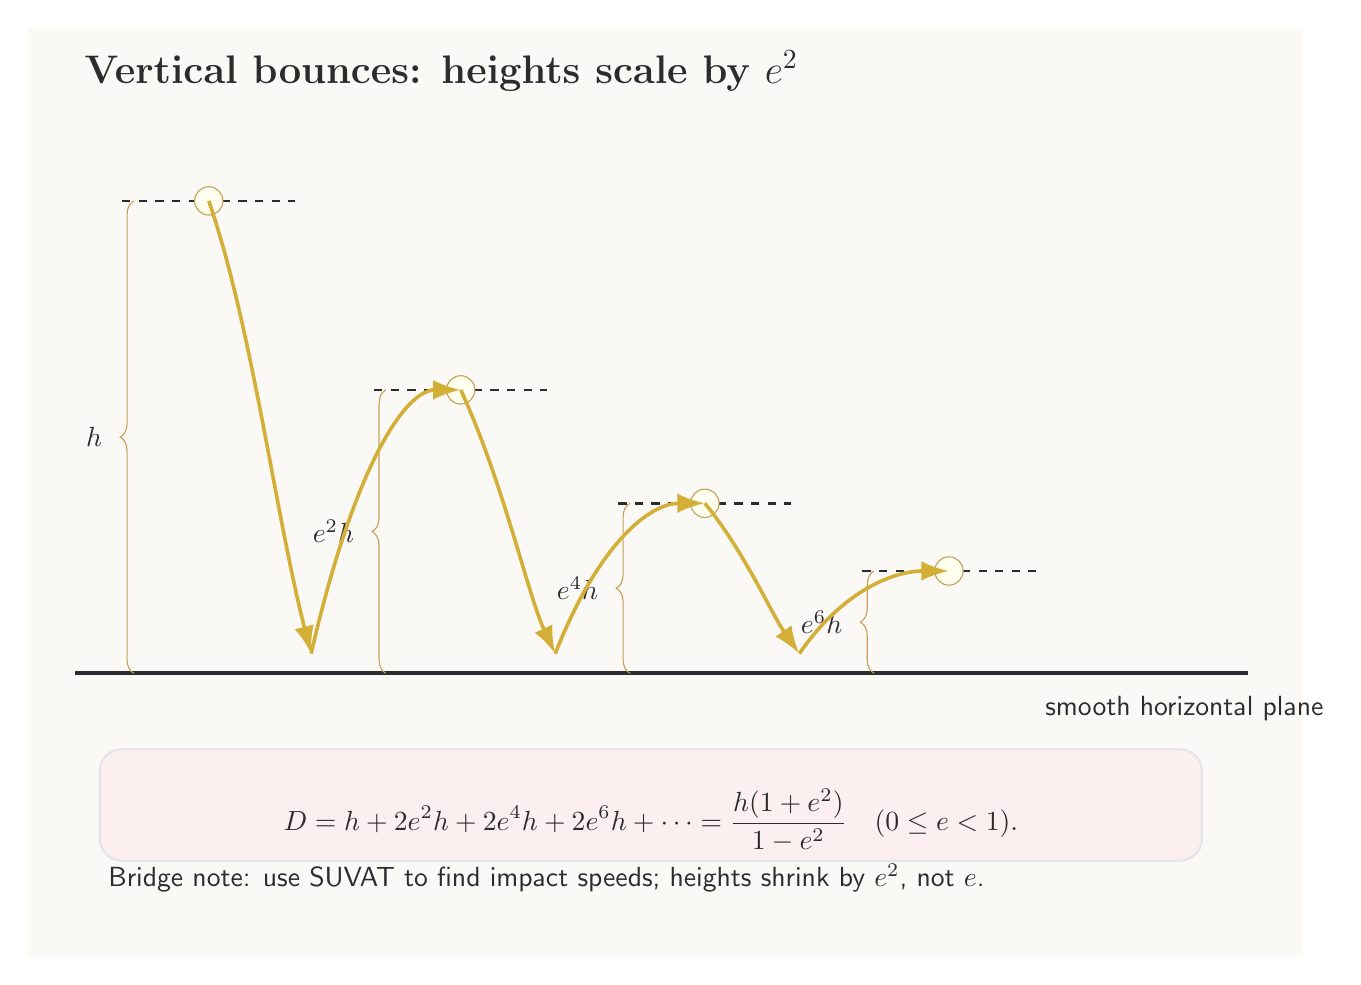
\begin{tikzpicture}[x=1cm,y=1cm,font=\sffamily,text=Ink]
\fill[Canvas] (-0.8,-3.6) rectangle (15.4,8.2);
\node[anchor=west,font=\bfseries\Large] at (-0.2,7.65) {Vertical bounces: heights scale by \(e^2\)};
\draw[Ink,line width=1.4pt] (-0.2,0)--(14.7,0);\node[anchor=west] at (12,-0.45) {smooth horizontal plane};
\draw[heightline] (0.4,6)--(2.6,6);\draw[heightline] (3.6,3.6)--(5.8,3.6);\draw[heightline] (6.7,2.16)--(8.9,2.16);\draw[heightline] (9.8,1.3)--(12,1.3);
\draw[decorate,decoration={brace,amplitude=5pt},draw=MutedGold] (0.55,0)--(0.55,6) node[midway,left=8pt] {\(h\)};
\draw[decorate,decoration={brace,amplitude=5pt},draw=MutedGold] (3.75,0)--(3.75,3.6) node[midway,left=8pt] {\(e^2h\)};
\draw[decorate,decoration={brace,amplitude=5pt},draw=MutedGold] (6.85,0)--(6.85,2.16) node[midway,left=8pt] {\(e^4h\)};
\draw[decorate,decoration={brace,amplitude=5pt},draw=MutedGold] (9.95,0)--(9.95,1.3) node[midway,left=8pt] {\(e^6h\)};
\filldraw[fill=Cream,draw=MutedGold] (1.5,6) circle (0.18);\filldraw[fill=Cream,draw=MutedGold] (4.7,3.6) circle (0.18);\filldraw[fill=Cream,draw=MutedGold] (7.8,2.16) circle (0.18);\filldraw[fill=Cream,draw=MutedGold] (10.9,1.3) circle (0.18);
\draw[bouncepath] (1.5,6)..controls (2.05,4.4) and (2.35,2)..(2.8,0.25);
\draw[bouncepath] (2.8,0.25)..controls (3.35,2.65) and (4,3.6)..(4.7,3.6);
\draw[bouncepath] (4.7,3.6)..controls (5.25,2.4) and (5.55,1)..(5.9,0.25);
\draw[bouncepath] (5.9,0.25)..controls (6.45,1.65) and (7.1,2.16)..(7.8,2.16);
\draw[bouncepath] (7.8,2.16)..controls (8.3,1.55) and (8.65,0.75)..(9,0.25);
\draw[bouncepath] (9,0.25)..controls (9.55,1.05) and (10.2,1.3)..(10.9,1.3);
\node[formulabox,minimum width=14cm,minimum height=1.35cm,anchor=north west] at (0.1,-0.95) {\begin{minipage}{13.4cm}\centering\[D=h+2e^2h+2e^4h+2e^6h+\cdots=\frac{h(1+e^2)}{1-e^2}\quad(0\le e<1).\]\end{minipage}};
\node[anchor=west] at (0.1,-2.6) {Bridge note: use SUVAT to find impact speeds; heights shrink by \(e^2\), not \(e\).};
\end{tikzpicture}
\end{document}
